\documentclass[12pt,letterpaper]{report}

% =============================================================================
% =  CUSTOM INFORMATION (stored as variables, used in template)
% =============================================================================

% The title of the paper.
\newcommand{\paperTitle}{My Thesis Title}

% The name of the author.
\newcommand{\paperAuthor}{Alison Major}

% The author's concentration in their Master of Science in Computer Science
\newcommand{\authorConcentration}{Software Engineering}

% =============================================================================
% =  PREAMBLE (packages and custom code)
% =============================================================================

\usepackage{paperPreamble}

% =============================================================================
% =  BEGINNING OF THE DOCUMENT
% =============================================================================

\begin{document}

% Include Page Numbers - Roman Numerals for Front Matter
\pagenumbering{roman}
\pagestyle{plain}

% =============================================================================
% =  Paper Title & Author Information
% =============================================================================

\begin{titlepage}
  \begin{center}
    
    \vfill
    
\includegraphics[width=0.8\textwidth]{UniversityLogo}
    
    \vspace{3cm}
    \large
    \textbf{\paperTitle}

    \vspace{0.5cm}
    A Thesis

    \vspace{0.5cm}
    By

    \vspace{0.5cm}
    \textbf{\paperAuthor}

    \vspace{2cm}
    Department of Computer and Mathematical Sciences

    \vspace{0.5cm}
    Submitted in partial fulfillment of the requirements

    \vspace{0.5cm}
    for the degree of \\
    Master of Science in Computer Science, 

    \vspace{0.5cm}
    Concentration in \authorConcentration

    \vspace{2cm}
    \today
          
  \end{center}
\end{titlepage}


% Set the document to be double spaced 
% http://kb.mit.edu/confluence/pages/viewpage.action?pageId=3907092
\doublespacing

% =============================================================================
% =  Signature Page
% =============================================================================

\newpage
\noindent
The undersigned have examined the thesis entitled `\textbf{\paperTitle}' presented by \textbf{\paperAuthor}, a candidate for the degree of \textbf{Master of Science in Computer Science (Concentration in \authorConcentration)} and hereby certify that it is worthy of acceptance.

\begin{center}
  \begin{tabularx}{1\textwidth} {
    >{\raggedright\arraybackslash}X
    m{1cm}
    m{3cm}
  }
    & & \\ & & \\ % Empty rows for spacing
    \cline{1-1} \cline{3-3}
    Advisor & & Date \\
    
    & & \\ & & \\ % Empty rows for spacing
    \cline{1-1} \cline{3-3}
    Program Director & & Date \\
    
    & & \\ & & \\ % Empty rows for spacing
    \cline{1-1} \cline{3-3}
    Department Chair & & Date 
  \end{tabularx}
\end{center}


% =============================================================================
% =  Paper Abstract
% =============================================================================

\newpage
\addcontentsline{toc}{section}{Abstract}
\section*{Abstract} \label{sectionAbstract}

% State the problem.
% Say why this problem is interesting.
% Say what my solution achieves.
% Say what follows from my solution.

All the pages have been formatted in the accepted font and margin alignment. This is a simple MS thesis template that can be used for directly typing in your content. However, if you paste your text into the document, do so with caution as pasting could produce varying results. When directly typing into the title page and signature page, the appropriate information should be filled in the required fonts.  If one chooses to include a copyright notice, it should appear before the signature page and after the title page (page ii). This can be achieved by clicking Insert > break > page break >ok.  Additionally, the page number should not appear on the copyright notice page. This can be achieved by clicking Insert > page numbers > format > start numbering at. I have used this thesis template to answer typical questions that grad students need addressed before they begin writing their theses. When writing an abstract, bare in mind an abstract is a short descriptive summary of your thesis. The number of words accepted might vary e.g. 200-250 words. An MS thesis abstract need not exceed two pages. \textbf{Abstracts are typically written last although they are the most important part of the thesis. They should have a little bit of everything: the background, the scope of your project, the purpose, findings and conclusions. An abstract is neither paragraphed nor cited. It should not be written as a literature review or a discussion of results. In a simplistic manner, your abstract, in a few words, should answer the questions: why should we care about your research; how did you get your results; what did you learn, find, create, invent; and finally what do your results imply?}

% =============================================================================
% =  Acknowledgements
% =============================================================================

\newpage
\addcontentsline{toc}{section}{Acknowledgements}
\section*{Acknowledgements} \label{sectionAcknowledgements}

% Remove the todo sections below.

Gratitude is a great virtue, though revenge is profitable

It's customary and good manners to say thank you however, where do you draw the line? In some of the theses that I've read, and I write this after having read thousands, literally, the following and more have been acknowledged: God, one's advisor, one's better half, parents, children, friends, classmates, lab-mates, lab technicians, lab assistants, pets, fav. Prof, neighbors, physicians, exercise trainer(s), wiki, the maintenance guy, landlord, the school hockey team, secretary, department head, driver, dentist, chauffer, the police, fav. presidential candidate, one's chef, Led Zeppelin, the pastor, one's biggest crush, the cable man, the mani/pedi girl, hair stylist, the best/worst/fav bar tender(s), the janitor, one's obs/gyn, one's mentor, and in a more recent thesis, Michael Phelps (8 gold medals at the 2008 Olympic games in Beijing, China, way to go...)

Keep in mind that one has to use one's own words when writing an acknowledgement. Plagiarism is unauthorized.

% =============================================================================
% =  Table of Contents
% =============================================================================

\newpage
\tableofcontents

% =============================================================================
% =  List of Tables
% =============================================================================

\newpage
\addcontentsline{toc}{section}{List of Tables}
\listoftables

% =============================================================================
% =  List of Figures
% =============================================================================

\newpage
\addcontentsline{toc}{section}{List of Figures}
\listoffigures

% =============================================================================
% =  Paper Content
% =============================================================================

% Include Page Numbers - Numbers (Arabic) for Main Matter
\pagenumbering{arabic}

% Chapter one defines the overall importance of the problem areas and provides an introduction into what you did.
\newpage
\chapter{Introduction} \label{sectionIntroduction}

The main goal of your introduction is to identify a problem that is worthy of investigation. It must also provide some idea of your research goals and approach to research.  Specific objectives can be introduced in the introduction chapter or they can be saved for later after you’ve provided additional background on the topic and state of the current research and its gaps.  The Introductory chapter often concludes with a summary of the organization of the thesis, including identification of the general content of specific chapters and appendices.

Ideally, chapter one defines the overall importance of the problem areas and provides an introduction into what you did, chapter two is why you did it in the context of what was previously known, three is how you did it, four is what you found and five is what it all means – putting the pieces together, (what’s your contribution to the research field).

It should be noted that the objectives of your research define the OUTCOME, i.e. what will be learned.  They are not a statement of the approach or tasks that are required to meet these objectives.  Some examples of reasonable research objectives:

\begin{itemize}
  \item Determine the effect of Marangoni convection on mixing of molten glasses
  \item Predict the extent of mechanical degradation of polymers
\end{itemize}

These both define the resulting outcome (prediction, effect on…) so they are objectives. The related tasks or research approach could be:

\begin{itemize}
  \item Solve a set of coupled non-linear PDEs\dots
  \item Perform experiments on\dots
\end{itemize}

These define the required steps; they do not define the outcome so they are NOT objectives.

Some theses and dissertations can have some chapters written as manuscripts that can be submitted to peer-reviewed scientific research journals. In that scenario, the grad student should be the principal author of the pending articles. The thesis or dissertation that includes manuscripts as chapters are not exempt from writing an introduction, background/ literature review and overall conclusions and recommendations.

This template uses the MS WORD STYLES extensively to help keep your work in the proper format.  These paragraphs use the “thesis-body text” style that is set for Times New Roman, 12 point font with double spaced lines and extra spacing between paragraphs (no need for hard carriage returns).  There are also styles for headers, equations, captions and bulleted lists that you can choose to use.  See examples throughout this template.


% Chapter two is why you did it in the context of what was previously known.
\newpage
\chapter{Background and Literature Review} \label{chapterBackground}

The background and literature review section needs to provide sufficient fundamental background information about the subject to support your objectives, hypothesis (or research questions) and methods, and review the pertinent literature related to the specific problem / hypothesis you are addressing. In Johnson (1991), some of the questions that he listed that the literature review should be to answer include: 

\begin{itemize}  
	\item what are the fundamental science, math, engineering concepts related to your research (scope),
	\item what part of your research work has ever been investigated before and what has not, (some of this may have been included in the introduction)
	\item how does your research work relate to that done by others, 
	\item how have others defined/measured/identified the key concepts of your research, 
	\item what data sources have you used or have other researchers used in developing general explanations for observed variations in a behavior or phenomenon in a concept in your thesis etc.  
\end{itemize}

The lit review (~20 pages or more) should not be limited to the above questions only. Ingeniousness and creativity is expected of a grad student.
Bullets can be single spaced.  The above bullets are in the style “thesis-bullets.”  When you type bulleted text, highlight the bulleted text and then select “thesis-bullets” from under the format, style menu to automatically change their formatting as above.

% include the section
\section{Section header}

Given the length of each chapter, it is required to use headers and sub headers (possibly sub-sub headers).  These can be numbered or one can just rely on different formats.  The section headers in this document are labeled “heading 2” (“heading 1” was used for chapter titles).  The heading styles formats should be consistent throughout the document as it helps significantly in creating the automatic table of contents.

\subsection{Sub Heading}

The subheadings here have a different format (“heading 3”) than the section headers.

\subsubsection{Sub-Sub Heading}

You can even get to another level of headers, defined here as “heading 4.”  The table of contents, however, is currently set up to just include three levels of headers.

\subsection{Equations}

Equations can be created in MS WORD equation editor or they can be created with other software.  Equations should be numbered.  They can be numbered within each chapter (e.g., 2.1, 2.2) or they can be numbered sequentially throughout the entire thesis.  Equations should be indented or centered with the equation number to the right.  The example below and associated “thesis-eqn” style can be used for all your equations.

\todo{Include example of an equation here.}

This equation was written with the equation editor. Found through “insert, object, equation editor 3.0. The equation editor can also be found through “tools, customize, commands”, and in categories, look for insert and in the commands section, look for equation editor, drag and drop the icon onto the toolbar. This editor is fine for relatively simple equations, other options are available for more complex equations.

\subsection{Tables}

Tables should have meaningful information with descriptive headers.  You can use the “thesis-table caption” style to define your captions and refer to the table in the text with a “cross reference” (Table 1).  MS Word re-numbers table captions automatically when new tables inserted.  But you need to right click on any cross references and “update field” if there are changes.

\begin{table}[h!]
  \centering
  \begin{tabularx}{0.8\textwidth} {
    | >{\centering\arraybackslash}X 
    | >{\centering\arraybackslash}X 
    | >{\centering\arraybackslash}X |
  }
    \hline
      Step \# & Instruction \\ 
    \hline
      Create table caption & Insert, reference, caption, table \\ 
    \hline
      Format the caption & Format, style, “thesis-table-caption” \\ 
    \hline
      Create table & Table, insert… \\
    \hline
      Format the table & The formatting of the table can vary, including use of single space as appropriate. Most journals require that tables are formatted using table style “Table Simple 1” format. \\
    \hline
      Reference the table from text & With the cursor at the location you want to cite the table: insert, reference, cross reference, table, label and number only. \\
    \hline
  \end{tabularx}
  \caption{Table 1: Steps in creating a table}
  \label{table:1}
\end{table}

\subsection{Figures}

Figures and illustrations are a necessary means of communicating technical information.  Often times, figures included in the background/lit review section are copied from existing copyrighted information.  In all cases, this is technically inappropriate without also receiving permission from the copyright owner.  Citing the source of the figure is not sufficient. This rule is enforced for PhD dissertations because they are submitted to ProQuest for electronic access by others.  The enforcement of this rule for MS theses is dependent on the specific committee members.

Resolution of figures is often a problem in theses.  Resolution should be >300 dpi, preferably 600dpi (\ref{fig:figure1}).  You should note that saving images as jpeg files is a sure way to lower the resolution to an unacceptable extent.  From experience, a good way is to copy your graphic (for example from PowerPoint or excel) and when pasting it into word, use the “paste special” “as an “enhanced metafile” (\ref{fig:figure2}).  This also substantially reduces the resulting file size in comparison with pasting graphs in as excel graphics.

\begin{figure}
  \centering
  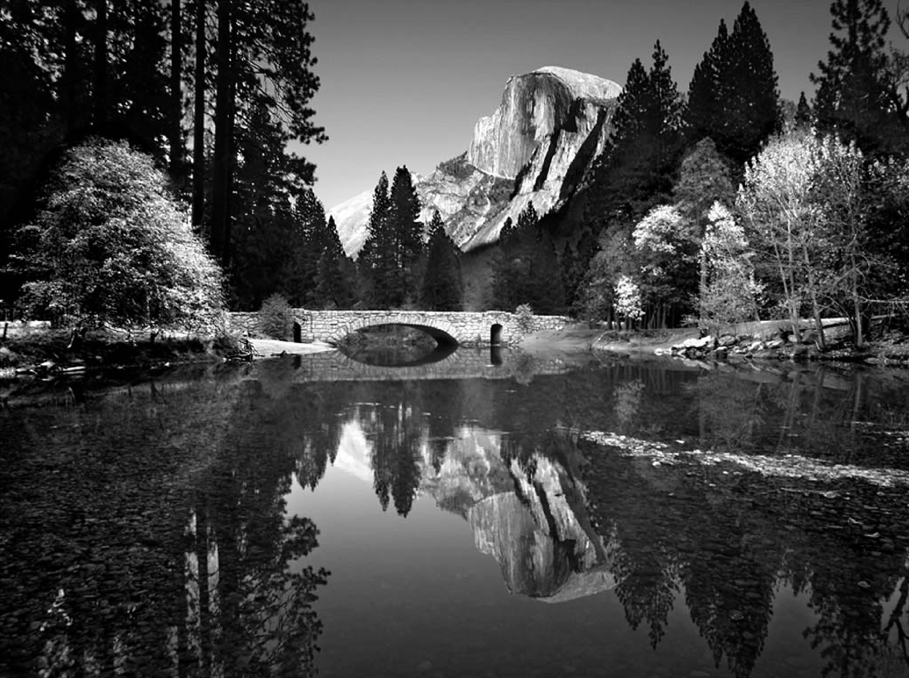
\includegraphics[width=0.8\textwidth]{Figure1}
  \caption{Figure 1: Example photo with high resolution.  Caption created with ``insert, reference, caption, figure'' and the style changed to ``thesis-figure caption.''}
  \label{fig:figure1}
\end{figure}

\begin{figure}
  \centering
  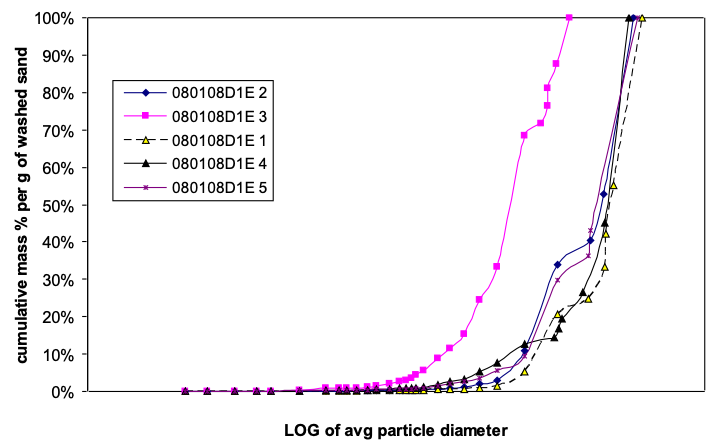
\includegraphics[width=0.8\textwidth]{Figure2}
  \caption{``Figure 2: Example of high resolution graphic inserted with “paste special, as enhanced metafile''}
  \label{fig:figure2}
\end{figure}


Sub heading (heading 3)
The subheadings here have a different format (“heading 3”) than the section headers.

Sub-sub heading (heading 4)
You can even get to another level of headers, defined here as “heading 4.”  The table of contents, however, is currently set up to just include three levels of headers.

Equations
Equations can be created in MS WORD equation editor or they can be created with other software.  Equations should be numbered.  They can be numbered within each chapter (e.g., 2.1, 2.2) or they can be numbered sequentially throughout the entire thesis.  Equations should be indented or centered with the equation number to the right.  The example below and associated “thesis-eqn” style can be used for all your equations.
		[1]
This equation was written with the equation editor. Found through “insert, object, equation editor 3.0. The equation editor can also be found through “tools, customize, commands”, and in categories, look for insert and in the commands section, look for equation editor, drag and drop the icon onto the toolbar. This editor is fine for relatively simple equations, other options are available for more complex equations.

Tables
Tables should have meaningful information with descriptive headers.  You can use the “thesis-table caption” style to define your captions and refer to the table in the text with a “cross reference” (Table 1).  MS Word re-numbers table captions automatically when new tables inserted.  But you need to right click on any cross references and “update field” if there are changes.
Table 1: Steps in creating a table

Figures
Figures and illustrations are a necessary means of communicating technical information.  Often times, figures included in the background/lit review section are copied from existing copyrighted information.  In all cases, this is technically inappropriate without also receiving permission from the copyright owner.  Citing the source of the figure is not sufficient. This rule is enforced for PhD dissertations because they are submitted to ProQuest for electronic access by others.  The enforcement of this rule for MS theses is dependent on the specific committee members.
Resolution of figures is often a problem in theses.  Resolution should be >300 dpi, preferably 600dpi (Figure 1).  You should note that saving images as jpeg files is a sure way to lower the resolution to an unacceptable extent.  From experience, a good way is to copy your graphic (for example from PowerPoint or excel) and when pasting it into word, use the “paste special” “as an “enhanced metafile” (Figure 2).  This also substantially reduces the resulting file size in comparison with pasting graphs in as excel graphics.

Figure 1: Example photo with high resolution.  Caption created with “insert, reference, caption, figure” and the style changed to “thesis-figure caption.”



Figure 2: Example of high resolution graphic inserted with “paste special, as enhanced metafile”

% Chapter three is how you did it.
\newpage
\chapter{Methodology} \label{chapterMethodology}

In addition to the detailed methods you need to describe in this section, you need to provide specific objectives and an overview of your approach if they have not already been presented in the introductory chapters.  The best place to put those items can vary among theses.  Sometimes the background and lit review is really necessary to justify and substantiate the specific objectives and approach and, therefore, it is best to save those details for the beginning of this chapter.

These paragraphs are in “thesis-body text.”  Other styles including captions, headers etc. can be used as presented in the previous chapter.  Table 2 summarizes all of the styles that can be used with this template.

\begin{table}[ht]
  \centering
  \begin{tabularx}{0.8\textwidth} {
    | >{\centering\arraybackslash}X 
    | >{\centering\arraybackslash}X |
  }
    \hline
      Style Name & When Used \\ 
    \hline\hline
      Heading 1 & Chapter Titles \\
      Heading 2 & Primary Headers \\
      Heading 3 & Sub Headers \\
      Heading 4 & Sub-Sub Headers \\
      Thesis-body text & All Paragraphs \\
      Thesis-bullets & Bullets \\
      Thesis Figure Caption & All figure captions. \\
      Thesis Table Caption & All table captions. \\
      Thesis-eqn & Equations \\
      Thesis-reference & Reference list at end of thesis \\
    \hline
  \end{tabularx}
  \caption{Table 2: Styles used in this template}
  \label{table:2}
\end{table}


% Chapter four is what you found.
\newpage
\chapter{Results} \label{chapterResults}

Results, findings, discussion of results OR manuscripts.  It is best to also reiterate information in your literature review to help substantiate the findings of your research.

This template is best used for directly typing in your content. 


% Chapter five is what it all means.
\newpage
\chapter{Conclusion} \label{chapterConclusion}

This chapter could also be called “Conclusions and Recommendations” or “Conclusions and Implications.” In general, there should be no new information presented here.  It should be a synthesis of information that you’ve already discussed. 


% =============================================================================
% =  References
% =============================================================================

\newpage
\begin{singlespace}
  \section*{References} \label{sectionReferences}

Includes all references: articles, media facts, books, reports, regulations, internet articles, papers that you referenced from the text.  In the text, citations can be (Smith and Jones, 2007) or Smith et al., 2007) (if more than two authors) if you wish to present your references alphabetically.  Alternatively, you can include the citations in the text as a number [1] or 1 if you wish to present your references numerically.  The MS WORD tools – “insert, reference, footnote, endnote” (or “cross reference” if you refer to the same reference more than once) should be used to help you organize and manage your references.

References can be written in single space with extra space between references as in the format below.  There are many different ways to arrange the information and punctuation in a reference listing.  The most important thing is to make sure all references are complete and that the format of your references is consistent throughout. 

Example, S.Z. (2008). How to cite a complete journal reference. J. Complete Thesis. 1(2): 47-52.

Example, S.Z., Second, W.S. (2007). How to cite a complete conference proceedings paper. In: Proceedings, 2nd International meeting of Masters Students, Paper \# XW15 (Potsdam NY, November, 2007).

If you use the “thesis” reference” style you will get the proper line spacing and indent style without further changes. Above are examples to show complete citation, other formats also acceptable.

\subsection*{Alternative format:}
An alternative format for references is to use IEEE format. You can find a reference on IEEE format here:  http://www.ijssst.info/info/IEEE-Citation-StyleGuide.pdf

You can use either the option provided above in the template or use the IEE format. 

We should cite something \cite{sample:docs}.

% =============================================================================
% =  Bibliography and Sources
% =============================================================================

\newpage
\bibliographystyle{IEEEtran}
\bibliography{bibliography}

\end{singlespace}

% =============================================================================
% =  Appendices
% =============================================================================

\newpage
\addcontentsline{toc}{section}{References}
\section*{Appendix A} \label{sectionAppendixA}

Type or paste your appendices here. Appendices are a place to organize and include all of the “extra” material that is important to your research work but that is too detailed for the main text.  Examples can include: specific analytical methods, computer code, spreadsheets of data, details of statistical analyses, etc.  But, these materials do not speak for themselves.  There should be a reference to these materials from the main chapters (complete details included in Appendix A) and there should be some text at the beginning of each appendix to briefly explain what the information is and means that is included in that appendix.


% =============================================================================
% =  Author Bibliography (Optional)
% =============================================================================

\newpage
% \begin{center}
  \large
  \textbf{BIBLIOGRAPHY}\footnote{IF NECESSARY (should not exceed one page except for PhDs)}
  
  
  \vspace{0.5cm}
  \textbf{\paperAuthor}

  \vspace{0.5cm}
  Candidate for the Degree of

  \vspace{0.5cm}
  Master of Science

\end{center}

\vspace{1cm}
Thesis: \MakeUppercase{\paperTitle}

\vspace{0.5cm}
Major Field: \authorConcentration

\vspace{0.5cm}
Biographical: \todo{fill something here}

\vspace{0.5cm}
Personal Data: \todo{fill something here}

\vspace{0.5cm}
Education: \todo{prior degrees}

\vspace{0.5cm}
``\paperAuthor'' has completed the requirements for the Master of Science in Computer Science at Lewis University, Romeoville, ILlinois, in ``\todo{Month}'', ``\todo{Year}''.

\vspace{1cm}
ADVISER'S APPROVAL: \todo{type adviser's name here}


% =============================================================================
% =  END OF THE DOCUMENT
% =============================================================================

\end{document}
